\section{Method}
\label{sec:prism-method}
% based on design, (callback 3.1) 1. text bridge
% subsubsection{1} have a brief intro, why align(difference between mindeye, solely text is enough), why use text xxx alignment
% subsection{2} the corresponding design: fmri text img. use a var as text, mlp, supervised by text

% compositional gene, existing insight: xxx, based on it we design
% formatting: 
%   then optimal object level description
% cross att

% prompt opt: auto text labeling, different prompt return different description. use llm to refine the keywords. the prompt can better label the images. then the description can be used to better recon

\vspace{-0.4cm}
\begin{figure}[t]
    \centering
    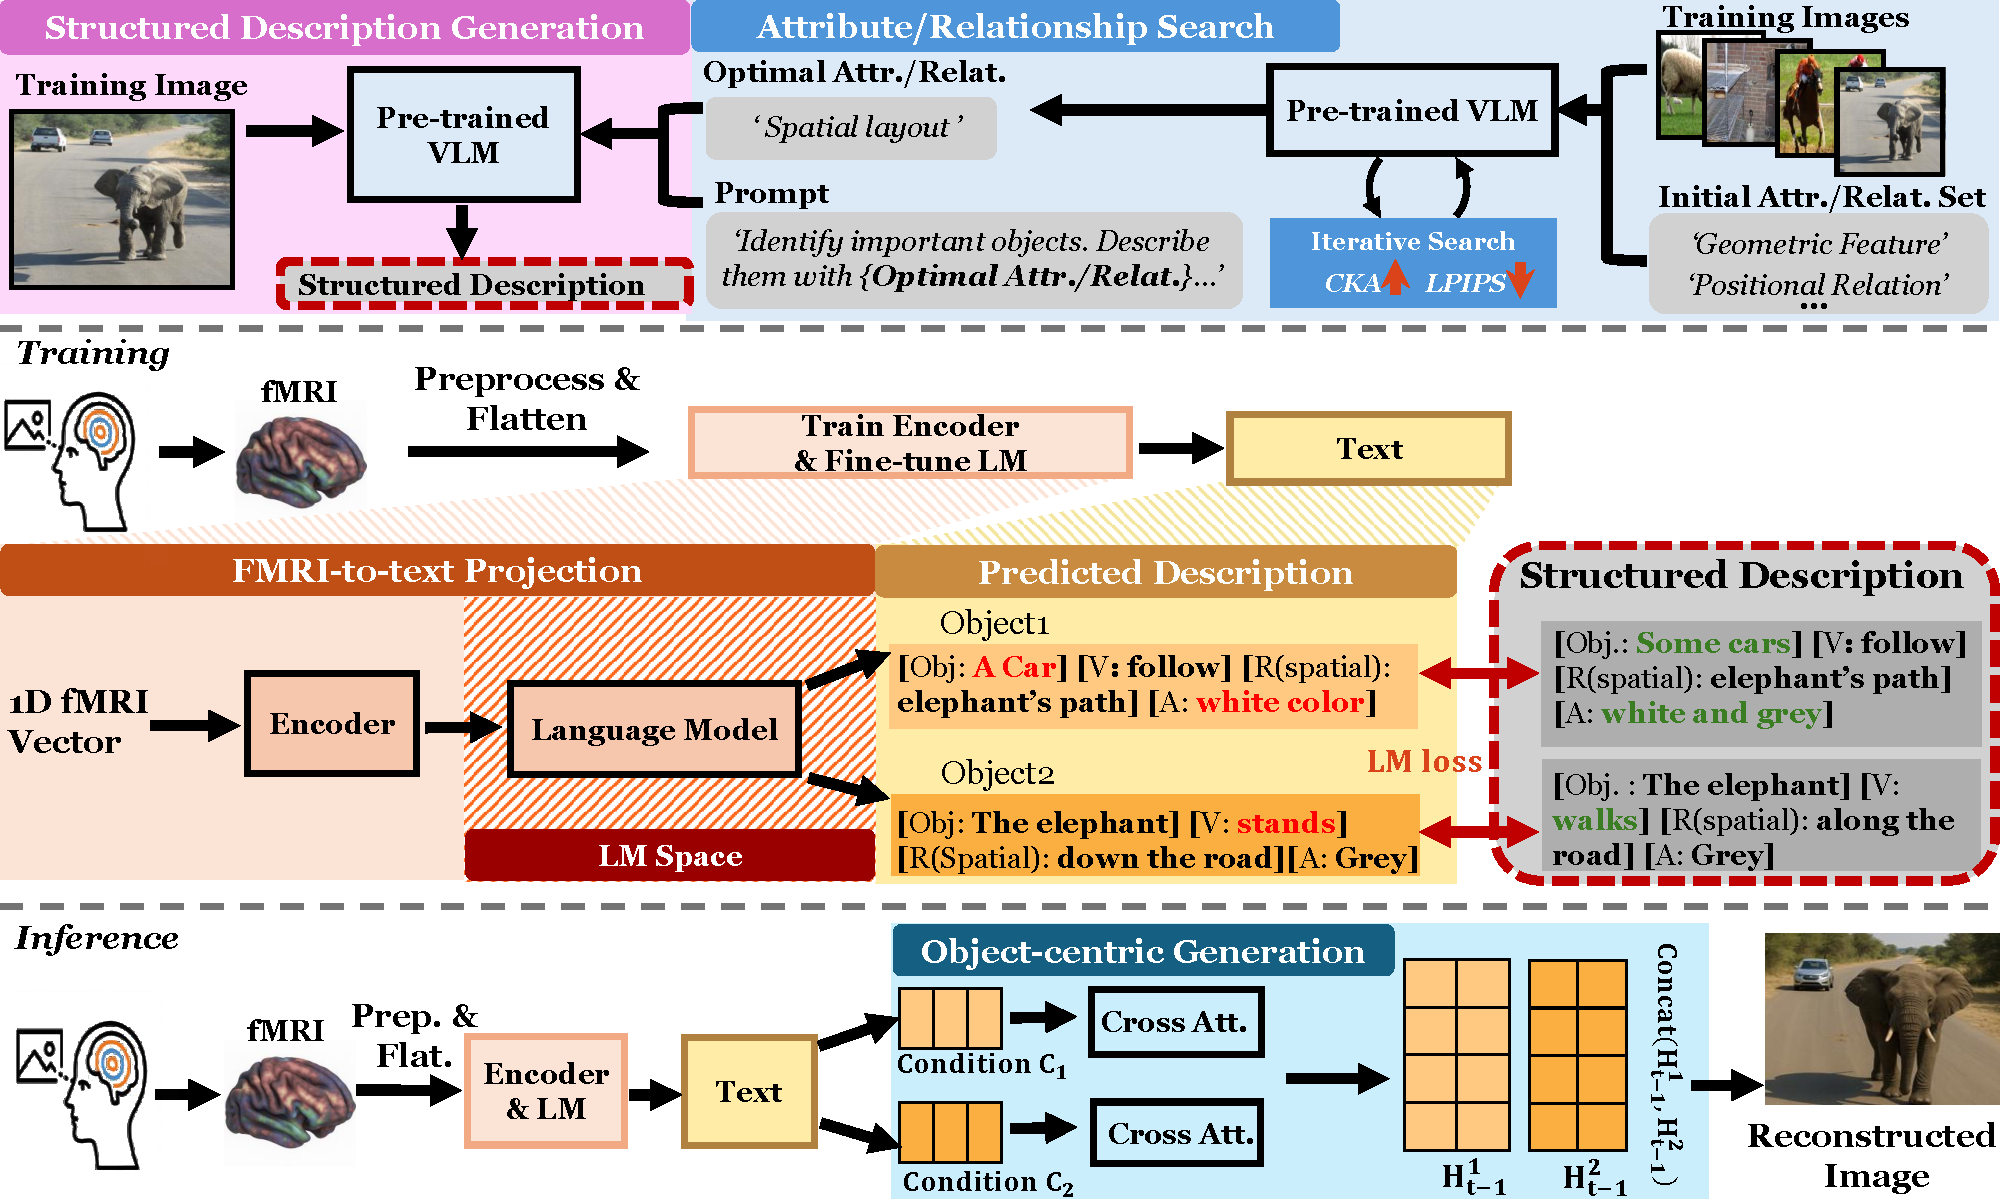
\includegraphics[width=0.98\linewidth]{figure/iclr_figure_new.pdf}
    \caption{\small Framework Overview: \modelname generates structured text descriptions for each training image using a VLM to iteratively extract brain-aligned object attributes and relationships. These descriptions capture the image’s compositional and relational content and serve as supervision to train an encoder and fine-tune a language model to map fMRI signals into the text space. During inference, the model predicts descriptions from fMRI signals, which then guide a pre-trained diffusion model for object-centric image reconstruction.}
    \label{fig:framework}
    \vspace{-0.25cm}
\end{figure}


In this section, we present our framework, \modelname, for fMRI-to-image reconstruction (Figure~\ref{fig:framework}). We first show that fMRI signals align most strongly with the text space of LMs, compared to the hidden spaces of vision or vision–language models, under established metrics (\Cref{sec:findings}). This finding motivates our choice of using pure text as the latent space.
During training (\Cref{sec: text_bridge}), we annotate each training image with structured text descriptions that are object-centric, compositional, and relational. To generate these descriptions, we introduce an attribute/relationship search module (\Cref{sec:train_desc_gen}), which learns optimal prompts to guide the VLM in automatically identifying the key attributes and relationships most aligned with both the fMRI signals and images. These structured descriptions are then used to train an encoder and fine-tune the LM, mapping fMRI signals into the LM text space (\Cref{sec:encoder_training}).
At inference time (\Cref{sec:inference}), the predicted structured descriptions guide an adapted diffusion model to generate object-centric images directly from fMRI signals.

% he framework comprises three key components: (1) Motivated by the finding that fMRI signals exhibit stronger alignment with LM text space under established metrics, we first project fMRI signals into the embedding space of a language model. 
% %Drawing on the compositional and object-centric nature of human visual perception, we guide image generation using structured, object-level descriptions. 
% (2) To reduce misattribution and better capture the object-based structure of perception, we constrain the text format used to condition generative models, designing structured descriptions that consist of objects and their attributes at multiple levels of detail.
% (3) To determine the most informative textual attributes, we formulate a prompt optimization problem for conditioning these descriptions. Each component is detailed in the following subsections.


% We begin by introducing the metrics used to quantify the similarity between fMRI data and various model representation spaces. 

%First, supported by neuroscientific findings that visual information transitions into an amodal semantic system near the visual cortex-and motivated by empirical evidence that fMRI signals align more closely with the text embeddings of language models-we propose to use the text space as a bridge to connect fMRI data and image generation. This is achieved by mapping the fMRI data to the text space of a language model. Second, inspired by the observation that human visual understanding is compositional and object-centric, we guide the image generation using structured, object-level decriptions. Finally, to understand what textual information should be provided to describe the object, we formulate a prompt optimization problem that searches for the optimal attribute to condition the structured descriptions. 

% \subsection{Design 1: Text Space as a Semantic Bridge from fMRI to Image Generation}
\subsection{Text as the Latent Space}
\label{sec:findings}
 We question whether using vision representations as the latent space is truly essential for reconstructing visual stimuli. In this section, we investigate the alignment between different model spaces and fMRI signals using various measures. 

\textbf{Measuring the alignment between model spaces and fMRI signals.}
We examine three representation spaces: (1) the text space of language models, (2) the joint text-image space of vision-language models, and (3) the latent space of vision models. For (2) and (3), image embeddings are extracted directly from the respective models. For (1), we use text embeddings from image captions to represent the stimuli. We extract embeddings by feeding either text or images into different models: T5 and LLaMA3
%\textcolor{blue}{Qwen3~\citep{yang2025qwen3}  and RoBERTa}~\citep{liu2019roberta} 
for text embeddings, 
%\textcolor{blue}{SD3}~\citep{esser2024scaling} 
LDM~\citep{rombach2022high} and ResNet50~\citep{he2016deep} for image embeddings, and CLIP for both modalities. 


Alignment is assessed using three metrics: Centered Kernel Alignment (CKA) \citep{murphy2024correcting}, Canonical Correlation Analysis (CCA)~\citep{wang2020finding}, and Generalization Gap~\citep{keskar2016large}. CKA and CCA are widely used to quantify similarity between representation spaces \citep{kriegeskorte2008representational, wang2020finding}. Generalization Gap reflects learnability by measuring the train-test loss difference when mapping fMRI signals to a target space using an MLP. Good alignment yields higher CKA and CCA values and a lower Generalization Gap.

Let \( \mathbf{X} = \text{Concat}(\mathbf{x}_1, \ldots, \mathbf{x}_N) \) denote concatenated fMRI samples and \( \mathbf{K} = \text{Concat}(\mathbf{k}_1, \ldots, \mathbf{k}_N) \) the corresponding latent representations. With \( \mathcal{K}(\cdot) \) as a kernel function, the empirical Hilbert-Schmidt Independence Criterion (HSIC) is:
\[
\text{HSIC}(\mathbf{X}, \mathbf{K}) = \frac{1}{(N - 1)^2} \operatorname{tr} \left( \mathcal{K}(\mathbf{X}) \cdot \mathcal{K}(\mathbf{K}) \right),
\]
where \( \operatorname{tr}(\cdot) \) denotes the trace operator. The CKA is the normalized form:
\[
\text{CKA}(\mathbf{X}, \mathbf{K}) = \frac{\text{HSIC}(\mathbf{X}, \mathbf{K})}{\sqrt{\text{HSIC}(\mathbf{X}, \mathbf{X}) \cdot \text{HSIC}(\mathbf{K}, \mathbf{K})}}.
\]
We adopt a Gaussian radial basis function (RBF) kernel for \( \mathcal{K} \) \citep{alvarez2022gaussian, cortes2012algorithms}. CCA identifies linear projections $\mathbf{u} = \mathbf{p}_1^\top \mathbf{X}$ and $\mathbf{v} = \mathbf{p}_2^\top \mathbf{K}$ that maximize their correlation. The first mode captures the dominant shared axis \citep{wang2020finding}, with the canonical correlation coefficient: $\rho = \text{corr}(\mathbf{u}, \mathbf{v}) = \text{corr}(\mathbf{p}_1^\top \mathbf{X}, \mathbf{p}_2^\top \mathbf{K}),$ reflecting the strongest linear alignment between brain activity and the model space.
\begin{wraptable}{r}{0.45\textwidth}  
\vspace{-0.2cm}
\centering
    \caption{\small Alignment results between model representations and fMRI data, evaluated using CKA, Generalization Gap, and CCA. The best result is highlighted in \textcolor{red}{red}. $\uparrow$ denotes higher is better; $\downarrow$ denotes lower is better.}
    \vspace{0.2cm}
    \resizebox{0.9\linewidth}{!}{

    \begin{tabular}{lccc}
    \toprule
               & \textbf{CKA} $\uparrow$   & \textbf{Generalization Gap}  $\downarrow$ & \textbf{CCA} $\uparrow$\\
    \midrule
    \textbf{T5}    & \textcolor{red}{0.5580}  & \textcolor{red}{0.1132}             &  \textcolor{red}{0.8344}   \\
    \textbf{Llama3} & 0.5442 & 0.2216             &  0.8022   \\
    \textbf{Clip text}  & 0.5177 & 0.4532             &   0.7599  \\
    \textbf{Clip img}   & 0.3668 & 0.4860                &   0.7573  \\
    \textbf{LDM}        & 0.1957 & 1.2520              & 0.7215    \\
    \textbf{Resnet50}     & 0.1822 & 1.9800               &  0.6746  \\
    \bottomrule

    \end{tabular}
    \label{tb_similarity}

    }
\vspace{-0.4cm}
\end{wraptable}

\textbf{FMRI aligns better with the embedding space of language models.} Our results (Table~\ref{tb_similarity}) show that the text space of language models aligns best with fMRI data, outperforming both vision–language and vision-only models across all metrics. Surprisingly, vision–language models, despite integrating both modalities, underperform compared to pure language models. We hypothesize that this is because humans focus more on the meaning of an image rather than pixel-level details~\citep{naselaris2009bayesian, du2022fmri}. Unlike prior work \citep{scotti2023reconstructing, wang2024decoding, xia2024dream, lin2022mind} that primarily relies on vision representations, our findings motivate using pure text as the latent space.





\subsection{Training of \modelname}
\label{sec: text_bridge}
% Building on our findings in \Cref{sec: finding_text}, we adopt the language model’s text space as a semantic bridge for fMRI-to-image generation. Our approach first maps fMRI signals into a language model’s embedding space and then generates textual descriptions that are subsequently linked to the vision model.
% In this section, we describe how PERM is trained to generate structured, object-level descriptions that capture the compositional nature of human visual perception.
In this section, we describe the training process of \modelname, which consists of automatic structured description generation for training images and encoder training.

\subsubsection{Automatic Description Generation}
\label{sec:train_desc_gen}
We design structured text descriptions as supervision for our framework. To capture the compositional and relational nature of human vision, these descriptions should explicitly distinguish between different objects and their relationships. Generating such descriptions with a VLM relies on carefully crafted prompts that specify the desired attributes and relationships, since many of them are not directly reflected in brain activity. To address this issue, we propose a VLM-assisted approach that automatically learns the most relevant attributes and relationships in an image based on the training data, ensuring they are both meaningful and brain-aligned.

%\yy{needs rewriting, notation issues, also, not only relationship, but also attribute, you can say a is a keyword, equation 1 useless}Given the $i$-th fMRI sample $\mathbf{x}_i \in \mathbb{R}^v$ and its corresponding stmimuli image's caption $D_i$\yy{not given}, 

We first show how structured descriptions can be generated from a VLM given a learned keyword $a$, and then present our approach for learning the optimal keyword. Given an image $\mathbf{Y}_i$ and a learned keyword $a$, we construct a prompt $\mathcal{P}(a)$ to guide the VLM in describing the most important objects in $\mathbf{Y}_i$ based on $a$. Formally, the VLM receives the image and the prompt as input and outputs a structured description $D_i^a$:
%(referred to as $D_i$ in \Cref{sec: text_bridge}):
\begin{equation}
    D_i^a = \text{VLM}(\mathbf{Y}_i, \mathcal{P}(a)).
%\vspace{-0.4cm}
\end{equation}

\vspace{-0.3cm}
The structured description is a list of $m$ object-level tuples along with background information:
% \vspace{-0.1cm}

\vspace{-0.3cm}
\begin{equation}
D_i^a = \left[ (o_1: d_1: \text{loc}_1), \; (o_2: d_2 : \text{loc}_2), \; \dots, \;( o_m: d_m: \text{loc}_m), bg_i \right].
% \vspace{-0.2cm}
\label{eq:structure_des}
\end{equation}

Each $o_j$ is an object in the image, $d_j$ is its description containing attributes and relationships with other objects conditioned on keyword $a$, and $\text{loc}_j$ denotes its location (selected from a predefined set). The term $bg_i$ represents the background information of image $\mathbf{Y}_i$. 
% This procedure ensures that the generated description is semantically structured, object-centric, and tailored to the chosen attribute. 
To ensure meaningful generation, we further augment each relation description $ d_j$ with a structured header encoding its semantic roles, following the PropBank annotation format~\citep{marquez2008semantic, he2017deep, ross2021tailor, palmer2005proposition}. \textcolor{black}{A case study on reconstruction with object-level description is provided in Section~\ref{app:case_obj_level} of the Appendix}.
%These headers annotate each sentence with argument structures,
%(e.g., [Obj], [V], [Attribute (A)], [Relationship (R)])
%as shown in Figure~\ref{fig:framework}.


% Object-level descriptions of training images are conditioned on a keyword $a$, which is expected to capture the attributes and relationships most relevant to brain activity. Since the choice of $a$ critically determines the semantic quality and neural alignment of the resulting descriptions, we cast keyword identification as a prompt optimization problem.
The choice of keyword $a$ strongly influences the attributes and relationships captured in the object descriptions, which in turn affects the quality of mapping fMRI signals to the text space. Ideally, these descriptions should capture the most important information shared between the fMRI signals and the stimulus images. To avoid manually selecting the keyword, we frame its discovery as a prompt optimization problem and introduce our attribute/relationship search module.
%Our objective is to identify the optimal keyword $a$ that produces high-quality descriptions $D_i^a$ for reconstructing the original image $\mathbf{Y}_i$.


%To investigate which attribute $a$ used by the VLM can generate the most effective descriptions $D_i^a$ to reconstruct the original image $I_i$, we formulate this challenge as a prompt optimization problem. 

Concretely, given a set of training images $\mathcal{Y}^{\text{train}} = \{\mathbf{Y}_1, \ldots, \mathbf{Y}_N\}$ and the corresponding fMRI signals $\mathcal{X}^{\text{train}} = \{\mathbf{x}_1, \ldots, \mathbf{x}_N\}$, we define the following optimization problem to find the optimal $a$ in the prompt ($\mathcal{P}(a)$) for the VLM:
\vspace{-0.2cm}
\begin{align}
\max_{a} \quad & \sum_{i=1}^N\mathcal{S}\left(\mathbf{Y}_i,\text{Diff}(\text{VLM}(\mathbf{Y}_i,\mathcal{P}(a)))\right) \label{eq:opt_obj} \\
\text{s.t.} \quad & \text{CKA}\left(\mathbf{X}, \mathbf{K}^a\right) > \beta; \nonumber\\
& \mathbf{X}=\text{Concat}(\mathbf{x}_1,\ldots,\mathbf{x}_N);~\mathbf{K}^a=\text{Concat}(\mathbf{k}_1^a,\ldots,\mathbf{k}_N^a); \nonumber\\
& \mathbf{k}_i^a = \text{LM}_{\text{ENC}}(\text{VLM}(\mathbf{Y}_i,\mathcal{P}(a)))~\text{for } i=1,\ldots,N \nonumber;
\end{align}
where $\mathcal{S}(\cdot, \cdot)$ denotes the similarity score between two images (e.g. negative perceptual loss); $\text{Diff}$ is a pre-trained diffusion model that generates images from captions produced by the VLM; $\text{Concat}$ indicates the concatenation operation across all training samples; and $\text{LM}_{\text{ENC}}$ is a pre-trained language model to encode captions generated by the VLM. The constraint enforces that the CKA similarity between the fMRI data $\mathbf{X}$ and the caption embeddings $\mathbf{K}^a$ generated using keyword $a$ exceeds a threshold $\beta$, ensuring strong alignment between the fMRI and text spaces. The objective ensures that descriptions derived from the optimal keyword support accurate reconstruction.

To optimize the keyword $a$ in~\Cref{eq:opt_obj}, we guide the search along semantic links: keywords with similar meanings tend to yield comparable reconstructions, so generating new keywords based on the semantic relationships of top-performing candidates helps uncover more effective prompt expressions. In the search, we utilize an LLM as a keyword generator and iteratively search for improved keywords in a step-by-step manner. We begin by initializing a keywords set $\mathcal{A}$ with a collection of frequently-used attribute and relationship keywords identified in prior works~\citep{johnson2015image,lu2016visual,krishna2017visual}. We expand $\mathcal{A}$ through an $\varepsilon$-greedy search strategy: at each search step, the keyword generator proposes new candidate keywords based on either the top-performing keywords in $\mathcal{A}$ with probability $1{-}\varepsilon$, or randomly selected keywords from $\mathcal{A}$ with probability $\varepsilon$. Only candidates that exceed the similarity threshold are added to $\mathcal{A}$. This balances refinement of effective keywords and exploration of diverse novel keywords. See Section~\ref{app:attr_opt} in the Appendix for the detailed algorithm and search results.





%and serve as ground-truth targets for training the encoder and fine-tuning the language model.



% Specifically, given the $i$-th fMRI sample $\mathbf{x}_i \in \mathbb{R}^v$ and its corresponding image caption $D_i$, we first train a neural encoder and fine-tune a language model (LM) to map $\mathbf{x}_i$ into the latent space of the LM, producing the ground truth caption. This caption is then transformed into the latent embeddings of a VLM (e.g. CLIP) and fed into a pre-trained prompt-conditioned diffusion model (Diff). The generated caption $\hat{D}_i$ and the reconstructed image $\hat{\mathbf{Y}}_i$ are:



% corresponding
% textual description $d$ of the image stimuli. Suppose its corresponding embeddings (a set of token embeddings) are given by $\mathbf{F}_i$, 
% Specifically, given a description $d$, which is a sequence of text for an image $I_i$ on attribute keyword $a$, we first map the fMRI signal $\mathbf{x}_{i} \in \mathbb{R}^v$ into $m$ embeddings using a MLP:
% \begin{equation}
%     \mathbf{f}_j= \text{MLP}_1(\mathbf{x}_{i}),
% \end{equation}
% $$
% \mathbf{z}_1, \mathbf{z}_2, \dots, \mathbf{z}_m = \text{MLP}_1(\mathbf{X}_{i}),
% $$


% Specifically, given a structured description consisting of $m$ objects, we map the fMRI signal $\mathbf{X}_{i} \in \mathbb{R}^v$ into $m$ embeddings using a MLP:
% $$
% \mathbf{z}_1, \mathbf{z}_2, \dots, \mathbf{z}_m = \text{MLP}_1(\mathbf{X}_{i}),
% % $$
% where $\mathbf{f}_i \in \mathbb{R}^{v'}$ is the latent embedding corresponding. Each embedding is subsequently transformed via another MLP into the input embedding space of a pre-trained language model (LM), which is then used to generate the description:

% where $\mathbf{f}_j \in \mathbb{R}^{v'}$ is the latent embedding corresponding to the $j$-th object. Each embedding is subsequently transformed via another MLP into the input embedding space of a pre-trained language model, which is then used to generate the structured descriptions:
% \begin{equation}
% \label{eq:d_i}
% \hat{d}_i = \text{LM}(\text{MLP}_2(\mathbf{z}_1, \dots, \mathbf{z}_m)).
% \end{equation}

% \begin{equation}
% \label{eq:d_i}
% \hat{D}_i^a = \text{LM}(\text{MLP}_2(\mathbf{z}_1, \dots, \mathbf{z}_m)).
% \end{equation}


% To ensure semantically meaningful generation, we augment each reference description $ d_i$  with a structured header that encodes its semantic roles, following the PropBank annotation format~\citep{marquez2008semantic, he2017deep, ross2021tailor, palmer2005proposition}. These headers label each sentence with argument structures (e.g., [Agent], [Action], [Patient]), as illustrated in Figure~\ref{fig:framework}, and are used as ground-truth targets during language model fine-tuning. The language model is optimized using a sum over \( m \) language modeling losses~\citep{chang2024survey, gunel2020supervised}:

% \begin{equation}
% \mathcal{L}_{\text{LM}} = - \sum_{j=1}^m \sum_{t'=1}^{T} \log p(y_{t'} \mid y_{<t'}, \mathbf{z}_j),
% \end{equation}

% where $ y_{t'}$ denotes the  $t'$-th token in the structured description with its corresponding header. This training strategy facilitates fine-grained semantic alignment between fMRI-derived representations and structured textual descriptions. We begin by training the MLPs independently for a fixed number of epochs, then fine-tune the language model and MLPs jointly to maximize overall reconstruction performance.



\subsubsection{Encoder Training}
\label{sec:encoder_training}
We design an encoder to map fMRI signals into the latent space of the language model, using structured and object-centric descriptions as supervision. Specifically, each object's information is independently encoded using an MLP. The resulting representations are concatenated and passed to the language model to generate estimated structured descriptions  $\hat{D}_i^a$, which can be expressed as:

% map the fMRI signals $x_i$ to each object's latent representation $\mathbf{f}_j$, concatnate these representations and feed to a 

% As a result, we are able to map fMRI signal $x_i$ into multiple objects' embeddings:
\vspace{-0.2cm}
% $$
% \mathbf{f}_1, \mathbf{f}_2, \dots, \mathbf{f}_m = \text{MLP}_1(\mathbf{x}_{i}),
% $$
% where $\mathbf{f}_j$ is the object's representation.  
% Specifically, the structured description can be predicted by:
\vspace{-0.3cm}
\begin{equation}
\label{eq:d_object}
\begin{split}
\mathbf{f}_j &= \text{MLP}_j(\mathbf{x}_{i}), \; j= 1, \cdots, m\\
    \hat{D}_i^a &= \text{LM}(\text{MLP}_g(\text{Concat}(\mathbf{f}_1, \dots, \mathbf{f}_m))),
\end{split}
\vspace{-0.2cm}
\end{equation}
% Consequently, the language model generates $m$ structured descriptions, each corresponding to an object in the image, along with a background description. The language model is thus optimized using a sum over $m$ language modeling losses~\citep{chang2024survey, gunel2020supervised}:
The language model is fine-tuned using a loss over all $m$ object descriptions~\citep{chang2024survey, gunel2020supervised}:
\vspace{-0.4cm}
\begin{equation}
\mathcal{L}_{\text{LM}} = - \sum_{j=1}^m \sum_{t'=1}^{T} \log p(y_{t'} \mid y_{<t'}, \mathbf{f}_j),
\end{equation}
where $ y_{t'}$ denotes the $t'$-th token in the structured description. This training strategy enables fine-grained alignment between fMRI signals and structured textual descriptions. We first train the MLPs independently for a fixed number of epochs, then jointly fine-tune the language model and MLPs to maximize overall reconstruction performance.



\subsection{\modelname Inference: Object-Centric Image Generation}
\label{sec:inference}
The inference process of \modelname has two steps: (1) generate structured descriptions $\hat{D}_i^a$ from fMRI signals using the trained encoder and language model, and (2) reconstruct the image by composing objects conditioned on these descriptions with a pre-trained diffusion model: $\hat{\mathbf{Y}}_i =\text{Diff}(\hat{D}_i^a)$. 
% \begin{equation}
% \label{eq:d}
% \begin{split}
%   %\hat{D}_i^a &= \text{LM} (\text{Encoder}(\mathbf{x}_{i})),\\
% \hat{\mathbf{Y}}_i &=\text{Diff}(\hat{D}_i^a).  
% \end{split}
% \vspace{-0.9cm}
% \end{equation}
% \vspace{-0.2cm}

To reflect the brain's compositional understanding of visual scenes, during inference, we adapt a pre-trained diffusion model to perform compositional image generation, inspired by~\citep{yang2024mastering}. Specifically,
given an image $\mathbf{Y}_i$ and its predicted structured description $\hat{D}_i^a$ (from~\Cref{eq:d_object}), we extract a set of predicted objects $\{o_j\}_{j=1}^m$ and a background description $\hat{bg}_i$. These are combined into a global context prompt $\hat{p}_0$ and embedded into a conditioning matrix $\mathbf{C}_0$. Similarly, each object description $\hat{d}_j$ is embedded into a corresponding conditioning matrix $\mathbf{C}_j$. These conditioning matrices guide the denoising process via cross-attention (\Cref{sec:prelim}) from time $t$ to 0. At each step, the hidden representation of object $j$ (or the global context when $j = 0$) at time $t-1$ is computed as: $\mathbf{H}_{t-1}^j = \text{CrossAttention}(\mathbf{H}_t, \mathbf{C}_j),$ where $\mathbf{H}_t$ is the hidden representation of the full image at time $t$. We then resize and concatenate the object representations according to their predicted locations $\hat{\text{loc}}_j$:
\begin{equation}
    \mathbf{H}_{t-1}^{\text{cat}}=\Psi(\{\mathbf{H}_{t-1}^j, \hat{\text{loc}}_j\}_{j=1}^m),
\end{equation}
where $\Psi(\cdot)$ denotes the resizing and spatially-aware concatenation operation. Thus, the image generation model encodes each object independently from its description and then spatially concatenates their hidden representations according to the predicted locations.
%\yy{one sentence to explain what is means as questioned in the rebuttal.}

To ensure smooth region boundaries and seamless fusion between objects and background, we compute a weighted sum of the global context latent and the object latents:
\begin{equation}
    \mathbf{H}_{t-1} = \beta \cdot \mathbf{H}_{t-1}^{\text{cat}} + (1 - \beta) \cdot \mathbf{H}_{t-1}^{0},
\end{equation}

where $\beta$ is a hyperparameter that controls the blending ratio. This process is repeated across denoising steps, enabling structured, object-aware generation aligned with the brain's visual understanding.

